\documentclass[man,floatsintext]{apa6}
\usepackage{lmodern}
\usepackage{amssymb,amsmath}
\usepackage{ifxetex,ifluatex}
\usepackage{fixltx2e} % provides \textsubscript
\ifnum 0\ifxetex 1\fi\ifluatex 1\fi=0 % if pdftex
  \usepackage[T1]{fontenc}
  \usepackage[utf8]{inputenc}
\else % if luatex or xelatex
  \ifxetex
    \usepackage{mathspec}
  \else
    \usepackage{fontspec}
  \fi
  \defaultfontfeatures{Ligatures=TeX,Scale=MatchLowercase}
\fi
% use upquote if available, for straight quotes in verbatim environments
\IfFileExists{upquote.sty}{\usepackage{upquote}}{}
% use microtype if available
\IfFileExists{microtype.sty}{%
\usepackage{microtype}
\UseMicrotypeSet[protrusion]{basicmath} % disable protrusion for tt fonts
}{}
\usepackage{hyperref}
\hypersetup{unicode=true,
            pdftitle={Satellite-detected drought frequencies predict plant life history strategies},
            pdfauthor={J. Grey Monroe, Brian Gill, Kathryn Turner, \& John K. McKay},
            pdfkeywords={drought adaptation, life history evolution, remote sensing,
phylogeography, herbaria records},
            pdfborder={0 0 0},
            breaklinks=true}
\urlstyle{same}  % don't use monospace font for urls
\usepackage{graphicx,grffile}
\makeatletter
\def\maxwidth{\ifdim\Gin@nat@width>\linewidth\linewidth\else\Gin@nat@width\fi}
\def\maxheight{\ifdim\Gin@nat@height>\textheight\textheight\else\Gin@nat@height\fi}
\makeatother
% Scale images if necessary, so that they will not overflow the page
% margins by default, and it is still possible to overwrite the defaults
% using explicit options in \includegraphics[width, height, ...]{}
\setkeys{Gin}{width=\maxwidth,height=\maxheight,keepaspectratio}
\IfFileExists{parskip.sty}{%
\usepackage{parskip}
}{% else
\setlength{\parindent}{0pt}
\setlength{\parskip}{6pt plus 2pt minus 1pt}
}
\setlength{\emergencystretch}{3em}  % prevent overfull lines
\providecommand{\tightlist}{%
  \setlength{\itemsep}{0pt}\setlength{\parskip}{0pt}}
\setcounter{secnumdepth}{0}
% Redefines (sub)paragraphs to behave more like sections
\ifx\paragraph\undefined\else
\let\oldparagraph\paragraph
\renewcommand{\paragraph}[1]{\oldparagraph{#1}\mbox{}}
\fi
\ifx\subparagraph\undefined\else
\let\oldsubparagraph\subparagraph
\renewcommand{\subparagraph}[1]{\oldsubparagraph{#1}\mbox{}}
\fi

%%% Use protect on footnotes to avoid problems with footnotes in titles
\let\rmarkdownfootnote\footnote%
\def\footnote{\protect\rmarkdownfootnote}


  \title{Satellite-detected drought frequencies predict plant life history
strategies}
    \author{J. Grey Monroe\textsuperscript{1,2}, Brian Gill\textsuperscript{3},
Kathryn Turner\textsuperscript{4}, \& John K. McKay\textsuperscript{2}}
    \date{}
  
\shorttitle{Drought and life history}
\affiliation{
\vspace{0.5cm}
\textsuperscript{1} Graduate Degree Program in Ecology, Colorado State University, Fort Collins, CO 80523, USA\\\textsuperscript{2} College of Agriculture, Colorado State University, Fort Collins, CO 80523, USA\\\textsuperscript{3} Institute for Environment and Society, Brown University, Providence, RI 02912, USA\\\textsuperscript{4} Biology Department, Pennsylvania State University, State College, PA 16802, USA}
\keywords{drought adaptation, life history evolution, remote sensing, phylogeography, herbaria records}
\usepackage{csquotes}
\usepackage{upgreek}
\captionsetup{font=singlespacing,justification=justified}

\usepackage{longtable}
\usepackage{lscape}
\usepackage{multirow}
\usepackage{tabularx}
\usepackage[flushleft]{threeparttable}
\usepackage{threeparttablex}

\newenvironment{lltable}{\begin{landscape}\begin{center}\begin{ThreePartTable}}{\end{ThreePartTable}\end{center}\end{landscape}}

\makeatletter
\newcommand\LastLTentrywidth{1em}
\newlength\longtablewidth
\setlength{\longtablewidth}{1in}
\newcommand{\getlongtablewidth}{\begingroup \ifcsname LT@\roman{LT@tables}\endcsname \global\longtablewidth=0pt \renewcommand{\LT@entry}[2]{\global\advance\longtablewidth by ##2\relax\gdef\LastLTentrywidth{##2}}\@nameuse{LT@\roman{LT@tables}} \fi \endgroup}


\usepackage{lineno}

\linenumbers
\newcommand{\beginsupplement}{\setcounter{table}{0}  \renewcommand{\thetable}{S\arabic{table}} \setcounter{figure}{0} \renewcommand{\thefigure}{S\arabic{figure}}}

\authornote{

Correspondence concerning this article should be addressed to J. Grey
Monroe, 307 University Ave, Fort Collins, CO 80523. E-mail:
\href{mailto:monroejg@colostate.edu}{\nolinkurl{monroejg@colostate.edu}}}

\abstract{
Explaining variation in life history strategies is a long-standing goal
of evolutionary biology. For plants, annual and perennial life histories
are thought to reflect adaptation to environments that differ in the
frequency of environmental stress such as drought. Here we test this
hypothesis in \textit{Heliophila} (Brassicaceae), a diverse genus of
flowering plants native to Southern Africa using herbarium occurrence
records and satellite-detected drought histories. We find that perennial
\textit{Heliophila} species are found in environments where droughts are
significantly less frequent compared to annuals. These associations are
predictive while controlling for phylogeny, lending support to the
hypothesis that drought related natural selection has influenced the
distributions of these strategies. Additionally, the difference in
drought frequency between annual and perennial species distributions is
greatest during the summer and fall, which also appears to be when
annuals are in the seed phase of their life cycle based on collection
dates of annual species. Together, these findings support traditional
hypotheses about the drivers of life history strategy in plants - that
perenniality is favored in environments with less frequent drought and
annuality in enviroments with more frequent drought by allowing them to
escape drought prone seasons as seeds. 
}

\usepackage{amsthm}
\newtheorem{theorem}{Theorem}[section]
\newtheorem{lemma}{Lemma}[section]
\theoremstyle{definition}
\newtheorem{definition}{Definition}[section]
\newtheorem{corollary}{Corollary}[section]
\newtheorem{proposition}{Proposition}[section]
\theoremstyle{definition}
\newtheorem{example}{Example}[section]
\theoremstyle{definition}
\newtheorem{exercise}{Exercise}[section]
\theoremstyle{remark}
\newtheorem*{remark}{Remark}
\newtheorem*{solution}{Solution}
\begin{document}
\maketitle

\hypertarget{introduction}{%
\section{Introduction}\label{introduction}}

\hypertarget{life-history-variation-in-plants}{%
\subsection{Life history variation in
plants}\label{life-history-variation-in-plants}}

Understanding the causes and consequences of life history variation is a
longstanding goal of ecology and evolutionary biology (Cole, 1954). In
plants, life histories are especially diverse, with herbaceous species
that complete their life cycle in a number of weeks to trees that live
for thousands of years (Brown, 1996). Along this continuum an important
division exists, distinguishing annuals (i.e.~monocarpic or semelparous)
which complete their seed to seed life cycle within a single calendar
year from perennials (i.e.~polycarpic or iteroparous{]} which can
persist over multiple years. Annual plants flower once, set seed,
senesce, and then die, spending at least some portion of the year as a
seed. In contrast, perennial plants can continue vegetative growth after
reproduction and experience all seasons. These represent fundamentally
different life history strategies, but the ecological factors that
explain their evolution remain uresolved (Friedman \& Rubin, 2015).

Identifying the drivers of selection for these alternative strategies is
important because annuals and perennials have differing impacts on
ecosystem functioning. For example, perennials have higher nitrogen
concentration and larger specific root length in annuals, which both
affect nutrient cycling (Garnier, Cordonnier, Guillerm, \& Sonié, 1997;
Roumet, Urcelay, \& Dı'az, 2006). Furthermore, predicting the conditions
that favor these strategies in nature is useful for developing more
sustainable perennial cropping systems (Lelièvre \& Volaire, 2009).

Classical theory predict shorter life spans and annuality in
environments where adult mortality is high (Charnov \& Schaffer, 1973;
Franco \& Silvertown, 1996; Stearns, 1992). In plants, this has been
extended to the hypothessis that annuality is adaptive when it allows
plants to escape drought (Schaffer \& M, 1975). Lack of water is perhaps
the greatest threat to survival during vegetatitive or reproductive
growth and annuals can remain dormant (and protected as a seed) during
drought. Thus, environments with greater seasonal drought frequency may
select for annual life histories that complete reproduction prior to
drought prone seasons. Conversely, environments with less frequent
drought may select for perennial species, which may benefit from
multiple bouts of reproduction and competitive advantage (Corbin \&
D'Antonio, 2004). These prediction has been supported by the association
of annualilty with arid environments in wild rice (Morishima, Sano, \&
Oka, 1984) and \emph{Oenothera} (Evans, Hearn, Hahn, Spangle, \&
Venable, 2005). Additionally, annual and perennial species of Nemesia
were qualitatively associated with winter rather and summer rainfall
environments respectively (Datson, Murray, \& Steiner, 2008) and annual
species of Scorzoneroides were associated with environments classified
as unpredictable (Cruz-Mazo, Buide, Samuel, \& Narbona, 2009). These
findings provide qualitative evidence supporting the prediction that
annual species are found in environments that experience more frequent
drought, and vice versa, but whether the history frequency of drought
events indeed predicts the distributions annual or perennial life
history strategies has yet to be tested.

Here we combine a long-term global dataset of satellite detected drought
events with metadata from natural collections to test these classic
hypotheses about the evolution of life history strategies within the
African endemic mustard genus, \emph{Heliophila} L. (Brassicaceae). If
annuallity is an adaptive strategy allowing plants to escape drought
prone seasons, then drought frequency should predict the distribution of
life history strategies across landscapes, and annual species should be
more commonly associated with drought prone regions than perennial
species. Furthermore, if annual species have adapted to escape drought
prone seasons as seeds, observations of annual species should be rare
during drought prone seasons. Phylogenetic relatedness can have
significant non-random effects on species distributions and life history
traits {[}{]}, and therefore we assessed the relationship between life
history distribution and drought frequency in a phylogenetically
controlled background.

\hypertarget{materials-and-methods}{%
\section{Materials and Methods}\label{materials-and-methods}}

\hypertarget{availability}{%
\subsection{Availability}\label{availability}}

All data and the source code to produce this manuscript are available at
\url{https://github.com/greymonroe/heliophila}.

\hypertarget{data}{%
\subsection{Data}\label{data}}

\hypertarget{satellite-detected-drought-data}{%
\subsubsection{Satellite-detected drought
data}\label{satellite-detected-drought-data}}

Remotely sensed data is a powerful tool for characterizing seasonal
patterns in drought because it is less limited in spatial and temporal
scope and resolution than weather stations or field observations
(AghaKouchak et al., 2015). To quantify the frequency of drought during
different seasons across landscapes, we used the remotely sensed
Vegetative Health Index (VHI), which measures landscape scale reductions
in plant cover and temperature conditions characteristic of drought
(Kogan, 2001). Generated from data collected by NOAA AVHRR satellites
since 1981, the VHI combines normalized difference vegetation index
(NDVI) derived measures of vegetative stress (Vegetative Condition Index
- VCI) with temperature stress indicated by anomalies in thermal spectra
(Temperature Condition Index - TCI).

The VHI of year \(y\) during week \(w\) of \([1,52]\) at pixel \(i\) is
derived from the following equations, where \(n\) is the number of years
observed.

\[VCI_{y,w,i} = 100\frac{NDVI_{y,w,i} - NDVI_{min}}{NDVI_{max} - NDVI_{min}}\]

where \(NDVI_{min} = min(NDVI_{1981,w,i}...NDVI_{1981+n,w,i})\) and
\(NDVI_{max} = max(NDVI_{1981,w,i}...NDVI_{1981+n,w,i})\)

\[TCI_{y,w,i} = 100\frac{T_{y,w,i} - T_{min}}{T_{max} - T_{min}}\]

where \(T_{min} = min(T_{1981,w,i}...T_{1981+n,w,i})\) and
\(T_{max} = max(T_{1981,w,i}...T_{1981+n,w,i})\)

\[VHI_{y,w,i} = 0.5(VCI_{y,w,i}) + 0.5(TCI_{y,w,i})\]

Thus, VHI measurements are standardized according to conditions
historically observed at each locations. These measurements have been
validated and generally used for evaluating drought risk and predicting
crop yields in agriculture (e.g., Rojas, Vrieling, \& Rembold, 2011;
Kogan et al., 2016). But they also present a tool to study seasonal
patterns in the frequency of drought across environments and to test
hypotheses about the effect of drought on ecological and evolutionary
processes. Indeed, the VHI has been applied recently to study drought
related ecology of natural species and proven useful for predicting
infraspecific variation in drought tolerance traits and genes
(Dittberner et al., 2018; Mojica et al., 2016; Monroe et al., 2018).
Here, we accessed VHI data at \(16km^2\) resolution from 1981 to 2015
(\url{https://www.star.nesdis.noaa.gov/smcd/emb/vci/VH/vh_ftp.php}) to
characterize the seasonal drought frequencies experienced by annual and
perennial \emph{Heliophila} sepecies.

\hypertarget{life-history-data-for-heliophila}{%
\subsubsection{Life history data for
Heliophila}\label{life-history-data-for-heliophila}}

\emph{Heliophila} is a genus of flowering plants endemic to the southern
portion of Africa including the Cape Floristic and Succulent Karoo
Regions. These are among the most botanically diverse environments on
Earth and the estimated \textasciitilde{}50 \emph{Heliophila} species
are considered to be the most diverse genus of the family Brassicaceae
(Mummenhoff, Al-Shehbaz, Bakker, Linder, \& Mühlhausen, 2005). This
genus includes both perennial and annual species and this change in life
history strategy has likely arisen multiple independent times (Appel \&
Al-Shehbaz, 1997; Mummenhoff et al., 2005). We used life histories
reported by Mummenhoff et al. (2005), grouping species with annual or
perennial life histories. Perenniality was defined based on the
traditional defition and included any form of perennial life history
(e.g., herbs, shrubs, mixed, etc).

\hypertarget{heliophila-herbarium-specimens}{%
\subsubsection{Heliophila herbarium
specimens}\label{heliophila-herbarium-specimens}}

Botanists have collected and maintained over 350 million botanical
specimens worldwide over the past 300 years. Herbarium specimens and
their associated metadata have been used since the 1960s to study
species' geographical distributions (reviewed by Willis et al. (2017)
and Lang, Willems, Scheepens, Burbano, and Bossdorf (2018)). And as they
become digitized (Soltis, 2017), these collections have been used to
study relationships between trait distributions, geography, and climate
(Davis, Willis, Connolly, Kelly, \& Ellison, 2015; Stropp et al., 2016;
Václavı'k, Beckmann, Cord, \& Bindewald, 2017; Wolf, Zimmerman,
Anderegg, Busby, \& Christensen, 2016). To characterize the diributions
of annual and perennial \emph{Heliophila} species, all records for the
genus \emph{Heliophila} were downloaded from the Global Biodiversity
Information Facility (gbif.org) on July 21, 2018.

\hypertarget{sequence-data-for-phylogeny}{%
\subsubsection{Sequence data for
phylogeny}\label{sequence-data-for-phylogeny}}

Aligned Heliophila ITS sequences were obtained from previous work by
Mandáková et al. (2012). Aethionema, Alliaria, Cardamine, Chamira, and
Rorippa ITS records from were downloaded from Genbank {[}{]} and aligned
together with Heliophila ITS sequences using MAFFT as outgroups {[}{]}.

\hypertarget{analyses}{%
\subsection{Analyses}\label{analyses}}

\hypertarget{drought-frequency-calculations}{%
\subsubsection{Drought frequency
calculations}\label{drought-frequency-calculations}}

To characterize drought regimens across the distrubtions of annual and
perennial species of \emph{Heliohpila}, we calculated drought during
different seasons at the location of observations for \emph{Heliophila}
records using the VHI. Specifically, we created global maps of the
frequencies of observing drought conditions (VHI\textless{}40, NOAA)
during the winter (quarter surrounding winter solstice), spring (quarter
surrounding spring equinox), summer (quarter surrounding summer
solstice) and fall (quarter surrounding fall equinox) from 1981 to 2015.
From these maps, the drought frequency during the winter, spring,
summer, and fall were extracted for the locations of all GBIF records.

\hypertarget{herbarium-record-quality-control}{%
\subsubsection{Herbarium record quality
control}\label{herbarium-record-quality-control}}

To remove instance with spurious location data, we filtered raw GBIF by
restricting our analyses to include only:\\
* Species with reported life history\\
* Records with geospatial data\\
* Records without known geospatial issues\\
* Records from collection sites classified as land pixels\\
* Records from Africa\\
* Non-duplicate records (ie. identical species, location, collection
date)

\hypertarget{phylogeny-construction}{%
\subsubsection{Phylogeny construction}\label{phylogeny-construction}}

Model selection for construction of phylogeny was performed in
jModeltest2 with CIPRES (cite). Based on this analysis, \(GTR + L\) were
selected. Ultrametric phylogeny was estimated with branch lengths as
relative time (details).

\hypertarget{comparison-of-drought-frequency-between-annual-and-perennial}{%
\subsubsection{Comparison of drought frequency between annual and
perennial}\label{comparison-of-drought-frequency-between-annual-and-perennial}}

To evaluate the hypothesis that annual and perennial life history
strategies reflect adaptations to alternative drought regimes, we tested
the corresponding prediction that the observed distributions of annual
and perennial \emph{Heliophila} species would be significantly
associated with historic drought frequency. The relationship between
drought frequencies across each taxon's range and life habitat (annual
or perennial) was evaluated using Firth's penalized-likelihood logistic
regression and phylogenetic logistic regression.

\hypertarget{collection-dates}{%
\subsubsection{Collection dates}\label{collection-dates}}

To test the hypothesis that annual species have adapted to escape
drought prone seasons as seeds, collection dates for herbarium specimens
were compared between annual and perennial species. Comparisons of
distributions were made by Two-sample Kolmogorov-Smirnov test, t-test,
and Barlett variance test.

\hypertarget{results}{%
\section{Results}\label{results}}

To test the hypothesis that annual and perennial plants reflect
adaptation to alternative drought environments we examined the landscape
distribution of life history strategies in the large and diverse mustard
genus, \emph{Heliophila} Figure \ref{fig:phylogeny}. Using both
herbarium specimen metadata and a 30 year dataset of satellite generated
climate information, we tested the prediction that annual species are
more often observed in drought-prone locations than perennial species,
when controlling for phylogenetic relatedness. We found that drought
frequency is significantly different between the distributions of annual
and perennial species, with annuals being found in environments with
significantly more frequent drought, and that this signal is strongest
during the summer. These results remain significant while controlling
for the phylogenetic relationships of Heliophila species, yielding
support for the role that natural selection has played in driving
contemporary distributions of these alternatives strategies in relation
to drought regimes.



\begin{figure}[!h]
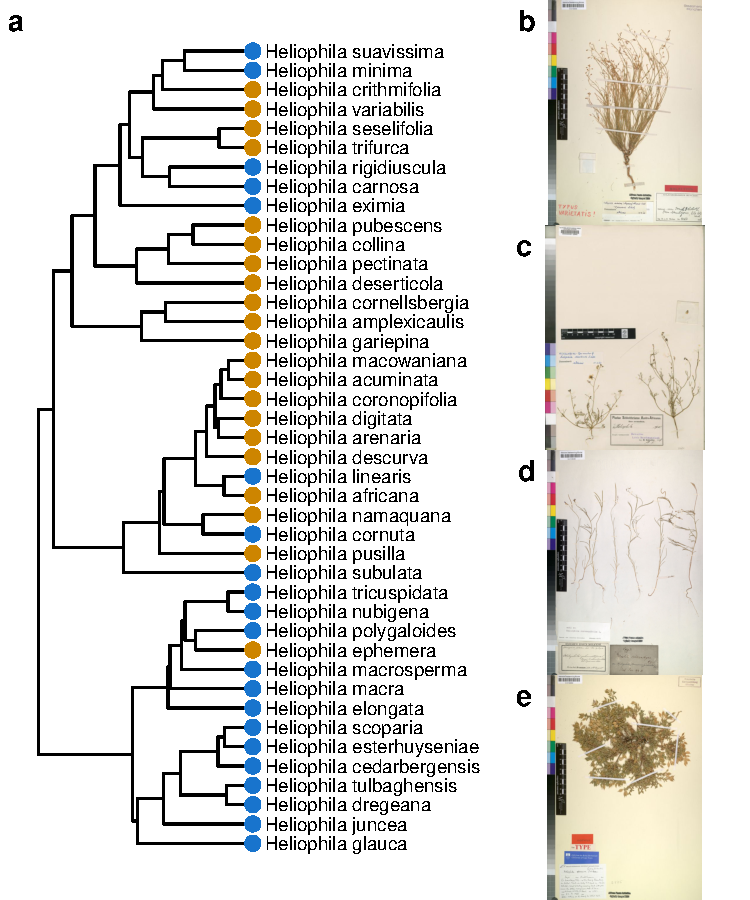
\includegraphics[width=\textwidth]{../figures/phylogeny} \caption{Phylogeny of Heliophila.}\label{fig:phylogeny}
\end{figure}

\hypertarget{gbif-records}{%
\subsubsection{GBIF records}\label{gbif-records}}

Out of 8670 \emph{Heliophila} GBIF recrods, 6634 were for species with
reported life history (Mummenhoff et al., 2005), 3653 had geospatial
data, 3627 did not have geospatial issues, 3460 were located on pixels
classified as land having drought measurements, 3457 were located in
Africa, 3162 were not duplicated. After all filtering steps, 2192
records for 42 species (Figure \ref{fig:mapsboxplots}, Table
\ref{tab:speciesmeanstable}) passed.

\hypertarget{drought-frequency}{%
\subsubsection{Drought frequency}\label{drought-frequency}}

Drought frequency was signicantly different between annual and perennial
species.






\begin{figure}[!h]
\includegraphics[width=\textwidth]{../figures/maps_boxplots} \caption{Locations of annual and perennial Heliophila. Drought
frequency during the winter, spring, summer and fall. Drought
frequencies during each season observed at the collection sites of
Heliophila records.}\label{fig:mapsboxplots}
\end{figure}

\begin{table}[tbp]
\begin{center}
\begin{threeparttable}
\caption{\label{tab:modelstable}Logistic regressions between life history, and the mean drought frequency observed at herbaria collection sites of Heliophila species the winter, spring, summer, and fall.}
\begin{tabular}{lllll}
\toprule
Predictor & \multicolumn{1}{c}{Estimate`} & \multicolumn{1}{c}{P`} & \multicolumn{1}{c}{Estimate*} & \multicolumn{1}{c}{P*}\\
\midrule
Intercept & 2.2575 & 0.1739 & 0.7231 & 0.6636\\
Winter drought freq. & -6.7484 & 0.1661 & -1.5452 & 0.7274\\ \midrule
Intercept & 4.5594 & 0.0443 & 5.0107 & 0.0534\\
Spring drought freq. & -11.7895 & 0.0423 & -12.9014 & 0.0464\\ \midrule
Intercept & 7.1742 & 0.0011 & 7.7093 & 0.0054\\
Summer drought freq. & -18.2999 & 0.0010 & -19.9056 & 0.0042\\ \midrule
Intercept & 6.4226 & 0.0029 & 7.0162 & 0.0082\\
Fall drought freq. & -19.0512 & 0.0026 & -20.8174 & 0.0067\\ \midrule
\bottomrule
\addlinespace
\end{tabular}
\begin{tablenotes}[para]
\normalsize{\textit{Note.} ` = Firth's penalized logistic regression. * = Phylogenetically constrained logistic regression. Annual species were scored as 0 and perennial species as 1.}
\end{tablenotes}
\end{threeparttable}
\end{center}
\end{table}

\hypertarget{collection-dates-1}{%
\subsubsection{Collection dates}\label{collection-dates-1}}






\begin{figure}
\centering
\includegraphics{../figures/line_and_dates.pdf}
\caption{\label{fig:lineplots}Comparison (mean +- SE) of drought frequency across
seasons measured at the GBIF records of annual and perennial species of
Heliophila. (B) Collection dates of GBIF records of annual and perennial
species of Heliophila.}
\end{figure}

\hypertarget{discussion}{%
\section{Discussion}\label{discussion}}

\hypertarget{summary}{%
\subsection{Summary}\label{summary}}

We found that the distribution of annual and perennial species of
Heliophila is significantly predicted by satellite detected historic
drought frequencies. Annual species are found in environments that
experience more frequent drought during the summer and fall quarters
compared to perennials. This relationship was consistent while
controlling for phylogenetic relatedness among the taxa studied,
indicating that these distributions cannot be explained entirely by
common ancestry. These results support the hypothesis that natural
selection has played a role in shaping the contemporary distributions of
these alternative life-history strategies.

\hypertarget{relationship-to-previous-hypotheseswork}{%
\subsection{Relationship to previous
hypotheses/work}\label{relationship-to-previous-hypotheseswork}}

Herbaria records and satellite detected drought provide data with which
the distributions of annual and perennial species can be compared with
respect to historic drought frequency. However, it is necessary to
control for the demographic history caused by common ancestry of species
if evolutionary processes such as natural selection are to be invoked as
explanations for any differences observed. If, for example, annual and
perennial species show significantly different ranges with respect to
historic drought this could be confounded by common ancestry if annuals
originated from a common ancestor and vice versa. In this case, it would
be challenging to distinguish between natural selection and demographic
history. On the other hand, if annual and perennial life history
strategies arose independently in multiple species, controlling for
phylogenetic relationships allows us to better account for demography
and make stronger assertions about the importance of processes such as
natural selection to explain patterns.

These findings support classical theoretical predictions about the
adaptive value of annual and perennial life history strategies. Taken
together, they suggest that in Heliophila, annual species are adapted to
environments with increased summer droughts by avoiding these seasons in
a dormant seed phase of their life cycle. Indeed, we found that very few
annuals are collected during this season, supporting the prediction that
they are not in a vegetative and/or reproductive phase at this time.
Traditionally, the focus has been on the evolutionary origins of annual
life histories \{citations\}. However, we also find evidence that the
transition to perenniality could be explained by historical drought
regimes. The phylogeny reveals several transitions from annual to
perennial life history. Perennials may be able to out complete annual
relatives in environments where the infrequency of drought favors
strategies that allow plants to benefit from growth over many seasons.

\hypertarget{caveats}{%
\subsection{Caveats}\label{caveats}}

Sampling bias (Daru et al., 2018). Correlation does not prove causation.
But it does indicate predictive power and is consistent with adaptive
hypotheses. Herbarium collections and their associated data do not
represent systematic or random sampling of a species distribution.
Significant biases in collecting exist, which we have not necessarily
controlled for here, and may have some effect on our findings, such as a
bias toward collecting near roads or near the locations of natural
history collections (Daru et al.~2018, Heberling, in press). Despite
these biases, the Cape Floristic region is a biodiversity hotspot and
one of the most botanically well sampled regions on Earth (Daru et
al.~2018, Heberling, in press?), suggesting that this may currently be
the optimal region for our analyses of life history distribution. Future
research will benefit from systematic sampling efforts to avoid these
noted biases. The climate data used here are assessed only from
198X-XXXX and do not reflect conditions at the estimated divergence
dates of these species (XXX million of years ago). Rather, the results
suggest that the current distributions of annual and perennial species
reflect a history of environmental filtration and ongoing natural
selection. That is, their distributions are non-random with respect to
historic drought and this is not explained by phylogeny.

\hypertarget{broader-implications}{%
\subsection{Broader implications}\label{broader-implications}}

These findings suggest that rapidly changing drought regimes threaten
species adapted to current environments. Studies predict changing
drought regimes. This could have impacts on ecosystem functioning. This
should also be considered when thinking about using perennial crops.
Studies predict changing drought regimes.

Do annuals require drought? We found independent origins of perenniality
in environments where droughts are infrequent. Annuals may not be able
to compete with perennials in the absence of droughts.

\hypertarget{conclusions}{%
\subsection{Conclusions}\label{conclusions}}

Perenniality appears to be adaptive in environments with less frequent
drought. This work demonstrates the power of emerging data to address
outstanding classic hypotheses in ecology and evolution.

\hypertarget{acknowledgments}{%
\section{Acknowledgments}\label{acknowledgments}}

This work was supported by NSF no. USDA grant no. XXX to J.G.M.

\hypertarget{references}{%
\section{References}\label{references}}

\newpage

\begingroup
\setlength{\parindent}{-0.5in}
\setlength{\leftskip}{0.5in}

\hypertarget{refs}{}
\leavevmode\hypertarget{ref-aghakouchak2015remote}{}%
AghaKouchak, A., Farahmand, A., Melton, F., Teixeira, J., Anderson, M.,
Wardlow, B. D., \& Hain, C. (2015). Remote sensing of drought: Progress,
challenges and opportunities. \emph{Reviews of Geophysics},
\emph{53}(2), 452--480.

\leavevmode\hypertarget{ref-R-geiger_a}{}%
Alfaro, M., Santini, F., Brock, C., Alamillo, H., Dornburg, A., Rabosky,
D., \ldots{} Harmon, L. (2009). Nine exceptional radiations plus high
turnover explain species diversity in jawed vertebrates.
\emph{Proceedings of the National Academy of Sciences of the United
States of America}, \emph{106}, 13410--13414.

\leavevmode\hypertarget{ref-appel1997generic}{}%
Appel, O., \& Al-Shehbaz, I. A. (1997). Generic limits and taxonomy of
hornungia, pritzelago, and hymenolobus (brassicaceae). \emph{Novon},
338--340.

\leavevmode\hypertarget{ref-R-papaja}{}%
Aust, F., \& Barth, M. (2018). \emph{papaja: Create APA manuscripts with
R Markdown}. Retrieved from \url{https://github.com/crsh/papaja}

\leavevmode\hypertarget{ref-R-Matrix}{}%
Bates, D., \& Maechler, M. (2018). \emph{Matrix: Sparse and dense matrix
classes and methods}. Retrieved from
\url{https://CRAN.R-project.org/package=Matrix}

\leavevmode\hypertarget{ref-brown1996oldlist}{}%
Brown, P. M. (1996). OLDLIST: A database of maximum tree ages.
\emph{Tree Rings, Environment, and Humanity. Radiocarbon}, \emph{1996},
727--731.

\leavevmode\hypertarget{ref-charnov1973life}{}%
Charnov, E. L., \& Schaffer, W. M. (1973). Life-history consequences of
natural selection: Cole's result revisited. \emph{The American
Naturalist}, \emph{107}(958), 791--793.

\leavevmode\hypertarget{ref-cole1954population}{}%
Cole, L. C. (1954). The population consequences of life history
phenomena. \emph{The Quarterly Review of Biology}, \emph{29}(2),
103--137.

\leavevmode\hypertarget{ref-corbin2004competition}{}%
Corbin, J. D., \& D'Antonio, C. M. (2004). Competition between native
perennial and exotic annual grasses: Implications for an historical
invasion. \emph{Ecology}, \emph{85}(5), 1273--1283.

\leavevmode\hypertarget{ref-cruz2009molecular}{}%
Cruz-Mazo, G., Buide, M., Samuel, R., \& Narbona, E. (2009). Molecular
phylogeny of scorzoneroides (asteraceae): Evolution of heterocarpy and
annual habit in unpredictable environments. \emph{Molecular
Phylogenetics and Evolution}, \emph{53}(3), 835--847.

\leavevmode\hypertarget{ref-daru2018widespread}{}%
Daru, B. H., Park, D. S., Primack, R. B., Willis, C. G., Barrington, D.
S., Whitfeld, T. J., \ldots{} others. (2018). Widespread sampling biases
in herbaria revealed from large-scale digitization. \emph{New
Phytologist}, \emph{217}(2), 939--955.

\leavevmode\hypertarget{ref-datson2008climate}{}%
Datson, P., Murray, B., \& Steiner, K. (2008). Climate and the evolution
of annual/perennial life-histories in nemesia (scrophulariaceae).
\emph{Plant Systematics and Evolution}, \emph{270}(1-2), 39--57.

\leavevmode\hypertarget{ref-davis2015herbarium}{}%
Davis, C. C., Willis, C. G., Connolly, B., Kelly, C., \& Ellison, A. M.
(2015). Herbarium records are reliable sources of phenological change
driven by climate and provide novel insights into species' phenological
cueing mechanisms. \emph{American Journal of Botany}, \emph{102}(10),
1599--1609.

\leavevmode\hypertarget{ref-dittberner2018natural}{}%
Dittberner, H., Korte, A., Mettler-Altmann, T., Weber, A., Monroe, G.,
\& Meaux, J. de. (2018). Natural variation in stomata size contributes
to the local adaptation of water-use efficiency in arabidopsis thaliana.
\emph{bioRxiv}, 253021.

\leavevmode\hypertarget{ref-R-geiger_b}{}%
Eastman, J., Alfaro, M., Joyce, P., Hipp, A., \& Harmon, L. (2011). A
novel comparative method for identifying shifts in the rate of character
evolution on trees. \emph{Evolution}, \emph{65}, 3578--3589.

\leavevmode\hypertarget{ref-evans2005climate}{}%
Evans, M. E., Hearn, D. J., Hahn, W. J., Spangle, J. M., \& Venable, D.
L. (2005). Climate and life-history evolution in evening primroses
(oenothera, onagraceae): A phylogenetic comparative analysis.
\emph{Evolution}, \emph{59}(9), 1914--1927.

\leavevmode\hypertarget{ref-franco1996life}{}%
Franco, M., \& Silvertown, J. (1996). Life history variation in plants:
An exploration of the fast-slow continuum hypothesis. \emph{Phil. Trans.
R. Soc. Lond. B}, \emph{351}(1345), 1341--1348.

\leavevmode\hypertarget{ref-friedman2015all}{}%
Friedman, J., \& Rubin, M. J. (2015). All in good time: Understanding
annual and perennial strategies in plants. \emph{American Journal of
Botany}, \emph{102}(4), 497--499.

\leavevmode\hypertarget{ref-garnier1997specific}{}%
Garnier, E., Cordonnier, P., Guillerm, J.-L., \& Sonié, L. (1997).
Specific leaf area and leaf nitrogen concentration in annual and
perennial grass species growing in mediterranean old-fields.
\emph{Oecologia}, \emph{111}(4), 490--498.

\leavevmode\hypertarget{ref-R-mvtnorm}{}%
Genz, A., \& Bretz, F. (2009). \emph{Computation of multivariate normal
and t probabilities}. Heidelberg: Springer-Verlag.

\leavevmode\hypertarget{ref-R-MCMCglmm}{}%
Hadfield, J. D. (2010). MCMC methods for multi-response generalized
linear mixed models: The MCMCglmm R package. \emph{Journal of
Statistical Software}, \emph{33}(2), 1--22. Retrieved from
\url{http://www.jstatsoft.org/v33/i02/}

\leavevmode\hypertarget{ref-R-geiger_d}{}%
Harmon, L., Weir, J., Brock, C., Glor, R., \& Challenger, W. (2008).
GEIGER: Investigating evolutionary radiations. \emph{Bioinformatics},
\emph{24}, 129--131.

\leavevmode\hypertarget{ref-R-logistf}{}%
Heinze, G., \& Ploner, M. (2018). \emph{Logistf: Firth's bias-reduced
logistic regression}. Retrieved from
\url{https://CRAN.R-project.org/package=logistf}

\leavevmode\hypertarget{ref-R-purrr}{}%
Henry, L., \& Wickham, H. (2018). \emph{Purrr: Functional programming
tools}. Retrieved from \url{https://CRAN.R-project.org/package=purrr}

\leavevmode\hypertarget{ref-R-raster}{}%
Hijmans, R. J. (2018). \emph{Raster: Geographic data analysis and
modeling}. Retrieved from
\url{https://CRAN.R-project.org/package=raster}

\leavevmode\hypertarget{ref-R-phylolm}{}%
Ho, L. S. T., \& Ane, C. (2014). A linear-time algorithm for gaussian
and non-gaussian trait evolution models. \emph{Systematic Biology},
\emph{63}, 397--408.

\leavevmode\hypertarget{ref-kogan2016modelling}{}%
Kogan, F., Guo, W., Strashnaia, A., Kleshenko, A., Chub, O., \&
Virchenko, O. (2016). Modelling and prediction of crop losses from noaa
polar-orbiting operational satellites. \emph{Geomatics, Natural Hazards
and Risk}, \emph{7}(3), 886--900.

\leavevmode\hypertarget{ref-kogan2001operational}{}%
Kogan, F. N. (2001). Operational space technology for global vegetation
assessment. \emph{Bulletin of the American Meteorological Society},
\emph{82}(9), 1949--1964.

\leavevmode\hypertarget{ref-lang2018using}{}%
Lang, P. L., Willems, F. M., Scheepens, J., Burbano, H. A., \& Bossdorf,
O. (2018). \emph{Using herbaria to study global environmental change}.
PeerJ Preprints.

\leavevmode\hypertarget{ref-lelievre2009current}{}%
Lelièvre, F., \& Volaire, F. (2009). Current and potential development
of perennial grasses in rainfed mediterranean farming systems.
\emph{Crop Science}, \emph{49}(6), 2371--2378.

\leavevmode\hypertarget{ref-mandakova2012whole}{}%
Mandáková, T., Mummenhoff, K., Al-Shehbaz, I. A., Mucina, L.,
Mühlhausen, A., \& Lysak, M. A. (2012). Whole-genome triplication and
species radiation in the southern african tribe heliophileae
(brassicaceae). \emph{Taxon}, \emph{61}(5), 989--1000.

\leavevmode\hypertarget{ref-Mojica2016}{}%
Mojica, J. P., Mullen, J., Lovell, J. T., Monroe, J. G., Paul, J. R.,
Oakley, C. G., \& McKay, J. K. (2016). Genetics of water use physiology
in locally adapted Arabidopsis thaliana. \emph{Plant Science}.
doi:\href{https://doi.org/10.1016/j.plantsci.2016.03.015}{10.1016/j.plantsci.2016.03.015}

\leavevmode\hypertarget{ref-monroe2018drought}{}%
Monroe, J. G., Powell, T., Price, N., Mullen, J., Howard, A., Evans, K.,
\ldots{} McKay, J. (2018). Drought adaptation in nature by extensive
genetic loss-of-function. \emph{bioRxiv}, 372854.

\leavevmode\hypertarget{ref-morishima1984differentiation}{}%
Morishima, H., Sano, Y., \& Oka, H. (1984). Differentiation of perennial
and annual types due to habitat conditions in the wild riceOryza
perennis. \emph{Plant Systematics and Evolution}, \emph{144}(2),
119--135.

\leavevmode\hypertarget{ref-mummenhoff2005phylogeny}{}%
Mummenhoff, K., Al-Shehbaz, I. A., Bakker, F. T., Linder, H. P., \&
Mühlhausen, A. (2005). Phylogeny, morphological evolution, and
speciation of endemic brassicaceae genera in the cape flora of southern
africa. \emph{Annals of the Missouri Botanical Garden}, 400--424.

\leavevmode\hypertarget{ref-R-bindrcpp}{}%
Müller, K. (2018). \emph{Bindrcpp: An 'rcpp' interface to active
bindings}. Retrieved from
\url{https://CRAN.R-project.org/package=bindrcpp}

\leavevmode\hypertarget{ref-R-tibble}{}%
Müller, K., \& Wickham, H. (2018). \emph{Tibble: Simple data frames}.
Retrieved from \url{https://CRAN.R-project.org/package=tibble}

\leavevmode\hypertarget{ref-R-caper}{}%
Orme, D., Freckleton, R., Thomas, G., Petzoldt, T., Fritz, S., Isaac,
N., \& Pearse, W. (2018). \emph{Caper: Comparative analyses of
phylogenetics and evolution in r}. Retrieved from
\url{https://CRAN.R-project.org/package=caper}

\leavevmode\hypertarget{ref-R-ape}{}%
Paradis, E., \& Schliep, K. (2018). Ape 5.0: An environment for modern
phylogenetics and evolutionary analyses in R. \emph{Bioinformatics},
\emph{xx}, xxx--xxx.

\leavevmode\hypertarget{ref-R-sp}{}%
Pebesma, E. J., \& Bivand, R. S. (2005). Classes and methods for spatial
data in R. \emph{R News}, \emph{5}(2), 9--13. Retrieved from
\url{https://CRAN.R-project.org/doc/Rnews/}

\leavevmode\hypertarget{ref-R-coda}{}%
Plummer, M., Best, N., Cowles, K., \& Vines, K. (2006). CODA:
Convergence diagnosis and output analysis for mcmc. \emph{R News},
\emph{6}(1), 7--11. Retrieved from
\url{https://journal.r-project.org/archive/}

\leavevmode\hypertarget{ref-R-gee}{}%
R by Thomas Lumley, V. J. C. P. to, \& author., B. R. N. that
maintainers are not available to give advice on using a package they did
not. (2015). \emph{Gee: Generalized estimation equation solver}.
Retrieved from \url{https://CRAN.R-project.org/package=gee}

\leavevmode\hypertarget{ref-R-base}{}%
R Core Team. (2018). \emph{R: A language and environment for statistical
computing}. Vienna, Austria: R Foundation for Statistical Computing.
Retrieved from \url{https://www.R-project.org/}

\leavevmode\hypertarget{ref-R-phytools}{}%
Revell, L. J. (2012). Phytools: An r package for phylogenetic
comparative biology (and other things). \emph{Methods in Ecology and
Evolution}, \emph{3}, 217--223.

\leavevmode\hypertarget{ref-R-maps}{}%
Richard A. Becker, O. S. code by, Ray Brownrigg. Enhancements by Thomas
P Minka, A. R. W. R. version by, \& Deckmyn., A. (2018). \emph{Maps:
Draw geographical maps}. Retrieved from
\url{https://CRAN.R-project.org/package=maps}

\leavevmode\hypertarget{ref-rojas2011assessing}{}%
Rojas, O., Vrieling, A., \& Rembold, F. (2011). Assessing drought
probability for agricultural areas in africa with coarse resolution
remote sensing imagery. \emph{Remote Sensing of Environment},
\emph{115}(2), 343--352.

\leavevmode\hypertarget{ref-roumet2006suites}{}%
Roumet, C., Urcelay, C., \& Dı'az, S. (2006). Suites of root traits
differ between annual and perennial species growing in the field.
\emph{New Phytologist}, \emph{170}(2), 357--368.

\leavevmode\hypertarget{ref-schaffer1975selection}{}%
Schaffer, W., \& M, G. (1975). Selection for optimal life histories in
plants. \emph{Ecology and Evolution of Communities.}, 142--157.

\leavevmode\hypertarget{ref-R-geiger_c}{}%
Slater, G., Harmon, L., Wegmann, D., Joyce, P., Revell, L., \& Alfaro,
M. (2012). Fitting models of continuous trait evolution to incompletely
sampled comparative data using approximate bayesian computation.
\emph{Evolution}, \emph{66}, 752--762.

\leavevmode\hypertarget{ref-R-diagram}{}%
Soetaert, K. (2017). \emph{Diagram: Functions for visualising simple
graphs (networks), plotting flow diagrams}. Retrieved from
\url{https://CRAN.R-project.org/package=diagram}

\leavevmode\hypertarget{ref-R-shape}{}%
Soetaert, K. (2018). \emph{Shape: Functions for plotting graphical
shapes, colors}. Retrieved from
\url{https://CRAN.R-project.org/package=shape}

\leavevmode\hypertarget{ref-soltis2017digitization}{}%
Soltis, P. S. (2017). Digitization of herbaria enables novel research.
\emph{American Journal of Botany}, \emph{104}(9), 1281--1284.

\leavevmode\hypertarget{ref-stearns1992evolution}{}%
Stearns, S. C. (1992). \emph{The evolution of life histories}.

\leavevmode\hypertarget{ref-stropp2016mapping}{}%
Stropp, J., Ladle, R. J., M. Malhado, A. C., Hortal, J., Gaffuri, J., H.
Temperley, W., \ldots{} Mayaux, P. (2016). Mapping ignorance: 300 years
of collecting flowering plants in africa. \emph{Global Ecology and
Biogeography}, \emph{25}(9), 1085--1096.

\leavevmode\hypertarget{ref-vaclavik2017effects}{}%
Václavı'k, T., Beckmann, M., Cord, A. F., \& Bindewald, A. M. (2017).
Effects of uv-b radiation on leaf hair traits of invasive
plants---combining historical herbarium records with novel remote
sensing data. \emph{PloS One}, \emph{12}(4), e0175671.

\leavevmode\hypertarget{ref-R-MASS}{}%
Venables, W. N., \& Ripley, B. D. (2002). \emph{Modern applied
statistics with s} (Fourth.). New York: Springer. Retrieved from
\url{http://www.stats.ox.ac.uk/pub/MASS4}

\leavevmode\hypertarget{ref-R-ggplot2}{}%
Wickham, H. (2016). \emph{Ggplot2: Elegant graphics for data analysis}.
Springer-Verlag New York. Retrieved from \url{http://ggplot2.org}

\leavevmode\hypertarget{ref-R-tidyverse}{}%
Wickham, H. (2017). \emph{Tidyverse: Easily install and load the
'tidyverse'}. Retrieved from
\url{https://CRAN.R-project.org/package=tidyverse}

\leavevmode\hypertarget{ref-R-forcats}{}%
Wickham, H. (2018a). \emph{Forcats: Tools for working with categorical
variables (factors)}. Retrieved from
\url{https://CRAN.R-project.org/package=forcats}

\leavevmode\hypertarget{ref-R-stringr}{}%
Wickham, H. (2018b). \emph{Stringr: Simple, consistent wrappers for
common string operations}. Retrieved from
\url{https://CRAN.R-project.org/package=stringr}

\leavevmode\hypertarget{ref-R-dplyr}{}%
Wickham, H., François, R., Henry, L., \& Müller, K. (2018). \emph{Dplyr:
A grammar of data manipulation}. Retrieved from
\url{https://CRAN.R-project.org/package=dplyr}

\leavevmode\hypertarget{ref-R-tidyr}{}%
Wickham, H., \& Henry, L. (2018). \emph{Tidyr: Easily tidy data with
'spread()' and 'gather()' functions}. Retrieved from
\url{https://CRAN.R-project.org/package=tidyr}

\leavevmode\hypertarget{ref-R-readr}{}%
Wickham, H., Hester, J., \& Francois, R. (2017). \emph{Readr: Read
rectangular text data}. Retrieved from
\url{https://CRAN.R-project.org/package=readr}

\leavevmode\hypertarget{ref-willis2017old}{}%
Willis, C. G., Ellwood, E. R., Primack, R. B., Davis, C. C., Pearson, K.
D., Gallinat, A. S., \ldots{} others. (2017). Old plants, new tricks:
Phenological research using herbarium specimens. \emph{Trends in Ecology
\& Evolution}, \emph{32}(7), 531--546.

\leavevmode\hypertarget{ref-wolf2016altitudinal}{}%
Wolf, A., Zimmerman, N. B., Anderegg, W. R., Busby, P. E., \&
Christensen, J. (2016). Altitudinal shifts of the native and introduced
flora of c alifornia in the context of 20th-century warming.
\emph{Global Ecology and Biogeography}, \emph{25}(4), 418--429.

\endgroup

\newpage
\setcounter{table}{0}  \renewcommand{\thetable}{S\arabic{table}} \setcounter{figure}{0} \renewcommand{\thefigure}{S\arabic{figure}}

\hypertarget{supplement}{%
\section{Supplement}\label{supplement}}

\hypertarget{software-used}{%
\subsubsection{Software used}\label{software-used}}

We used R (Version 3.5.1; R Core Team, 2018) and the R-packages
\emph{ape} (Version 5.2; Paradis \& Schliep, 2018; Orme et al., 2018;
Soetaert, 2018), \emph{bindrcpp} (Version 0.2.2; Müller, 2018),
\emph{caper} (Version 1.0.1; Orme et al., 2018), \emph{coda} (Version
0.19.2; Plummer, Best, Cowles, \& Vines, 2006), \emph{diagram} (Version
1.6.4; Soetaert, 2017), \emph{dplyr} (Version 0.7.8; Wickham et al.,
2018), \emph{forcats} (Version 0.3.0; Wickham, 2018a), \emph{gee}
(Version 4.13.19; R by Thomas Lumley \& author., 2015), \emph{geiger}
(Version 2.0.6; Alfaro et al., 2009; Eastman, Alfaro, Joyce, Hipp, \&
Harmon, 2011; Harmon, Weir, Brock, Glor, \& Challenger, 2008; Slater et
al., 2012), \emph{ggplot2} (Version 3.1.0; Wickham, 2016),
\emph{logistf} (Version 1.23; Heinze \& Ploner, 2018), \emph{maps}
(Version 3.3.0; Richard A. Becker, Ray Brownrigg. Enhancements by Thomas
P Minka, \& Deckmyn., 2018), \emph{MASS} (Version 7.3.51.1; Venables \&
Ripley, 2002), \emph{Matrix} (Version 1.2.15; Bates \& Maechler, 2018),
\emph{MCMCglmm} (Version 2.26; Hadfield, 2010), \emph{mvtnorm} (Version
1.0.8; Genz \& Bretz, 2009), \emph{papaja} (Version 0.1.0.9842; Aust \&
Barth, 2018), \emph{phylolm} (Version 2.6; Ho \& Ane, 2014),
\emph{phytools} (Version 0.6.60; Revell, 2012), \emph{purrr} (Version
0.2.5; Henry \& Wickham, 2018), \emph{raster} (Version 2.8.4; Hijmans,
2018), \emph{readr} (Version 1.2.1; Wickham et al., 2017), \emph{shape}
(Version 1.4.4; Soetaert, 2018), \emph{sp} (Version 1.3.1; Pebesma \&
Bivand, 2005), \emph{stringr} (Version 1.3.1; Wickham, 2018b),
\emph{tibble} (Version 1.4.2; Müller \& Wickham, 2018), \emph{tidyr}
(Version 0.8.2; Wickham \& Henry, 2018), and \emph{tidyverse} (Version
1.2.1; Wickham, 2017) for all our analyses.

\hypertarget{supplementary-tables-and-figures}{%
\subsubsection{Supplementary tables and
figures}\label{supplementary-tables-and-figures}}

\begin{center}
\begin{ThreePartTable}
\begin{TableNotes}[para]
\normalsize{\textit{Note.} LH = Life history (a = annual, p = perennial). n=sample size of GBIF records. Seasons are mean drought frequencies observed at locations of records.}
\end{TableNotes}
\small{
\begin{longtable}{lllllll}\noalign{\getlongtablewidth\global\LTcapwidth=\longtablewidth}
\caption{\label{tab:speciesmeanstable}Heliophila species records and the mean drought frequencies during different seasons at the location of records }\\
\toprule
Species & \multicolumn{1}{c}{LH} & \multicolumn{1}{c}{n} & \multicolumn{1}{c}{Winter} & \multicolumn{1}{c}{Spring} & \multicolumn{1}{c}{Summer} & \multicolumn{1}{c}{Fall}\\
\midrule
Heliophila acuminata & a & 28 & 0.32 & 0.38 & 0.41 & 0.36\\
Heliophila africana & a & 91 & 0.33 & 0.35 & 0.34 & 0.34\\
Heliophila amplexicaulis & a & 60 & 0.32 & 0.36 & 0.39 & 0.33\\
Heliophila arenaria & a & 65 & 0.34 & 0.37 & 0.38 & 0.34\\
Heliophila carnosa & p & 129 & 0.33 & 0.37 & 0.39 & 0.31\\
Heliophila cedarbergensis & p & 3 & 0.40 & 0.43 & 0.32 & 0.27\\
Heliophila collina & a & 16 & 0.35 & 0.47 & 0.48 & 0.45\\
Heliophila cornellsbergia & a & 2 & 0.33 & 0.42 & 0.35 & 0.21\\
Heliophila cornuta & p & 101 & 0.35 & 0.40 & 0.40 & 0.34\\
Heliophila coronopifolia & a & 40 & 0.37 & 0.42 & 0.40 & 0.37\\
Heliophila crithmifolia & a & 97 & 0.35 & 0.42 & 0.45 & 0.38\\
Heliophila descurva & a & 12 & 0.36 & 0.38 & 0.38 & 0.29\\
Heliophila deserticola & a & 133 & 0.48 & 0.48 & 0.46 & 0.45\\
Heliophila digitata & a & 30 & 0.33 & 0.38 & 0.44 & 0.38\\
Heliophila dregeana & p & 17 & 0.33 & 0.37 & 0.33 & 0.32\\
Heliophila elongata & p & 82 & 0.26 & 0.32 & 0.30 & 0.25\\
Heliophila ephemera & a & 3 & 0.14 & 0.27 & 0.31 & 0.26\\
Heliophila esterhuyseniae & p & 3 & 0.21 & 0.30 & 0.37 & 0.27\\
Heliophila eximia & p & 12 & 0.42 & 0.41 & 0.32 & 0.34\\
Heliophila gariepina & a & 12 & 0.50 & 0.53 & 0.48 & 0.41\\
Heliophila glauca & p & 35 & 0.29 & 0.35 & 0.34 & 0.33\\
Heliophila juncea & p & 150 & 0.32 & 0.37 & 0.39 & 0.35\\
Heliophila linearis & p & 94 & 0.32 & 0.33 & 0.28 & 0.30\\
Heliophila macowaniana & a & 31 & 0.33 & 0.38 & 0.44 & 0.39\\
Heliophila macra & p & 22 & 0.30 & 0.30 & 0.32 & 0.29\\
Heliophila macrosperma & p & 5 & 0.28 & 0.36 & 0.35 & 0.25\\
Heliophila minima & p & 35 & 0.36 & 0.45 & 0.51 & 0.39\\
Heliophila namaquana & a & 16 & 0.39 & 0.46 & 0.48 & 0.39\\
Heliophila nubigena & p & 19 & 0.31 & 0.36 & 0.43 & 0.38\\
Heliophila pectinata & a & 16 & 0.27 & 0.34 & 0.50 & 0.34\\
Heliophila polygaloides & p & 12 & 0.40 & 0.48 & 0.42 & 0.34\\
Heliophila pubescens & a & 9 & 0.31 & 0.40 & 0.48 & 0.39\\
Heliophila pusilla & a & 45 & 0.32 & 0.38 & 0.38 & 0.34\\
Heliophila rigidiuscula & p & 201 & 0.30 & 0.33 & 0.28 & 0.24\\
Heliophila scoparia & p & 106 & 0.31 & 0.37 & 0.36 & 0.31\\
Heliophila seselifolia & a & 80 & 0.36 & 0.42 & 0.45 & 0.40\\
Heliophila suavissima & p & 92 & 0.30 & 0.39 & 0.42 & 0.31\\
Heliophila subulata & p & 103 & 0.29 & 0.33 & 0.31 & 0.29\\
Heliophila tricuspidata & p & 8 & 0.28 & 0.33 & 0.38 & 0.30\\
Heliophila trifurca & a & 77 & 0.45 & 0.48 & 0.48 & 0.43\\
Heliophila tulbaghensis & p & 3 & 0.36 & 0.41 & 0.36 & 0.35\\
Heliophila variabilis & a & 97 & 0.35 & 0.41 & 0.40 & 0.37\\
\bottomrule
\addlinespace
\insertTableNotes
\end{longtable}
}
\end{ThreePartTable}
\end{center}


\end{document}
